\documentclass[sigconf]{acmart}
\usepackage{arydshln}

\usepackage{booktabs} % For formal tables


% Copyright
\setcopyright{none}
\settopmatter{printacmref=false}
%\setcopyright{acmcopyright}
%\setcopyright{acmlicensed}
%%\setcopyright{rightsretained}
%\setcopyright{usgov}
%\setcopyright{usgovmixed}
%\setcopyright{cagov}
%\setcopyright{cagovmixed}
\setlength{\belowcaptionskip}{-17pt}

%% DOI
%\acmDOI{10.475/123_4}
%
%% ISBN
%\acmISBN{123-4567-24-567/08/06}
%
%%:Conference
\acmConference[]{}{}{}
%\copyrightyear{2016}
%
%\acmArticle{4}
%\acmPrice{15.00}

% These commands are optional
%\acmBooktitle{Transactions of the ACM Woodstock conference}
%\editor{Jennifer B. Sartor}
%\editor{Theo D'Hondt}
%\editor{Wolfgang De Meuter}


\begin{document}
\title{Towards Dynamic Load Balancing Policies\\in Software-Defined Storage}
%\titlenote{Produces the permission block, and
%  copyright information}
%\subtitle{Extended Abstract}
%\subtitlenote{The full version of the author's guide is available as
%  \texttt{acmart.pdf} document}

\author{Michael A. Sevilla, Carlos Maltzahn}
\affiliation{\institution{University of California, Santa Cruz}}
%\email{{msevilla, carlosm}@soe.ucsc.edu}

\makeatother
\author{Bradley W. Settlemyer, Danny Perez, David Rich, Galen M. Shipman (LANL)}
%\email{{bws, danny_perez, dor, gshipman}@lanl.gov}

\begin{abstract}

Our analysis of the key-value activity generated under multiple initial
conditions, demonstrates the need for a distributed, load balancing key-value
store for the ParSplice molecular dynamics simulation.  Our analysis indicates
the presence of clear access regimes and hot spots that offer significant
opportunity for optimization. We then leverage the Mantle load balancing
framework, which was originally designed for distributed file systems, to
dynamically switch policies and present a two policy scheme that achieves 93\%
efficiency while using only 1\% of the memory resources required by the base
case. Finally, we demonstrate how a machine learning clustering technique is an
effective method for detecting access patterns within the keyspace over time.  

\end{abstract}

%
% The code below should be generated by the tool at
% http://dl.acm.org/ccs.cfm
% Please copy and paste the code instead of the example below. 
%
%\begin{CCSXML}
%<ccs2012>
% <concept>
%  <concept_id>10010520.10010553.10010562</concept_id>
%  <concept_desc>Computer systems organization~Embedded systems</concept_desc>
%  <concept_significance>500</concept_significance>
% </concept>
% <concept>
%  <concept_id>10010520.10010575.10010755</concept_id>
%  <concept_desc>Computer systems organization~Redundancy</concept_desc>
%  <concept_significance>300</concept_significance>
% </concept>
% <concept>
%  <concept_id>10010520.10010553.10010554</concept_id>
%  <concept_desc>Computer systems organization~Robotics</concept_desc>
%  <concept_significance>100</concept_significance>
% </concept>
% <concept>
%  <concept_id>10003033.10003083.10003095</concept_id>
%  <concept_desc>Networks~Network reliability</concept_desc>
%  <concept_significance>100</concept_significance>
% </concept>
%</ccs2012>  
%\end{CCSXML}

%\ccsdesc[500]{Computer systems organization~Embedded systems}
%\ccsdesc[300]{Computer systems organization~Redundancy}
%\ccsdesc{Computer systems organization~Robotics}
%\ccsdesc[100]{Networks~Network reliability}
%
%
%\keywords{ACM proceedings, \LaTeX, text tagging}


\maketitle

\section{Introduction}

\begin{itemize}
  \item key-value stores
  \begin{enumerate}
    \item Fine scale annotation
    \item Scalability
    \item flexible, extensible formats
  \end{enumerate}
  \item science
  \begin{enumerate}
    \item entropy is increasing
    \item graph showing regimes (key distribution, popularity over time)
  \end{enumerate}
\end{itemize}

Hypothesis: re-distributing keys requires dynamic load balancing policies\cite{perez:jctc20150parsplice}



%% What is the problem?
%Load balancing is a useful tool for optimizing performance in systems that
%service highly accessed data\footnote{In this paper, we use the term ``data" to
%refer to the partitioned key-value pairs AND file system metadata.} but
%deciding how to make the migrations is a risky trade-off. In this paper, we
%show that a one-size-fits-all data load balancing policy is not sufficient for
%even the simplest of HPC applications and argue for a dynamic load balancing
%policy.
%
%% Explain techniques
%Resource migration is the key mechanism for load balancing. In storage, data
%can be distributed to alleviate overloaded servers or it can be concentrated to
%exploit locality. These techniques are at odds and selecting the wrong
%technique can have catastrophic consequences. For example, migrating data to an
%already overloaded server or increasing the network hops by spreading data
%across an underutilized cluster will impact performance negatively.
%
%% Why is concentration vs. distribution difficult?
%Unfortunately, deciding which optimization to use is difficult to reason about,
%especially with the scale and complexity of today's HPC architectures. While
%the mechanisms are usually built into the systems, the policies often times
%less refined and much more sensitive to the workload. So a system may have the
%ability exploit locality using techniques like bulk operations, multiple
%partition strategies, secondary indexes, and caching but deciding when, where,
%and how to use them is workload dependent and difficult to figure out.
%
%% What we did in the paper
%This paper takes an API designed to migrate file system metadata and applies it
%to an HPC key-value store.  The API helps control distribution and
%concentration by letting the administrator define how to migrate load, where to
%migrate load, and how much load to migrate. While designed for a different
%domains, this API encompasses many of the same properties we need for an HPC
%key-value store, namely:
%
%\begin{itemize}
%  \item services small/frequent requests
%  \item popularity drives distribution
%  \item locality drives concentration
%\end{itemize}
%
%\begin{figure}[t]
%  \noindent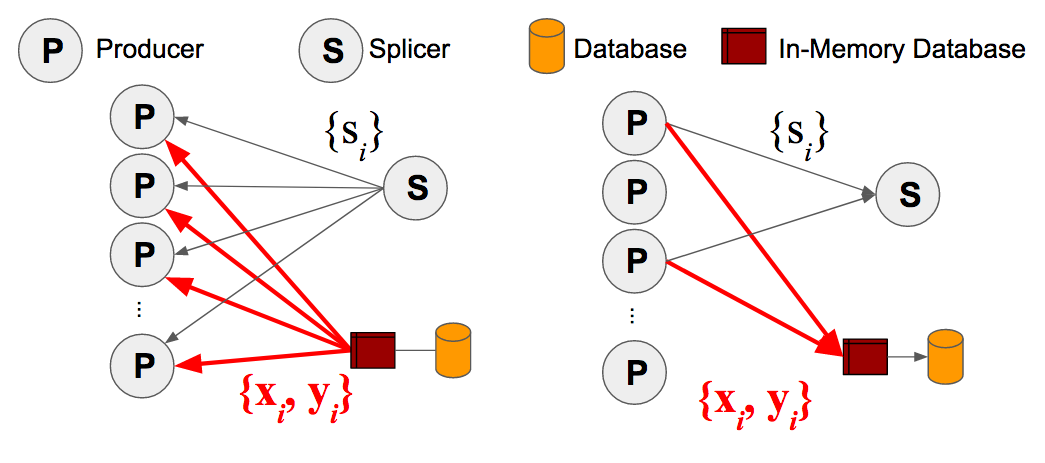
\includegraphics[width=19pc,angle=0]{figures/arch-parsplice.png}\\
%  \caption{ParSplice is a ready-heavy HPC application where producers use a
%  database for consistency. Replacing the single-node database with HXHIM
%  improves performance with load balancing.
%  \label{fig:arch-parsplice}}
%\end{figure}
%
%% Why is HXHIM a good fit?
%To show the efficacy of this approach, we examine the ParSplice molecular
%dynamics simulation application shown in Figure~\ref{fig:arch-parsplice}.
%ParSplice uses a single-node database for consistency, where producers, \(P\),
%push and pull coordinates, \{\(x_i, y_i\)\}, based on the segments,
%\{\(s_i\)\}, assigned by the splicer, \(S\). In this paper, we replace the
%database with a distributed key-value store designed for HPC enjoy performance
%optimizations for:
%
%\begin{itemize}
%  \item \texttt{put()} because of the distributed sync and load balancing based on:
%  \begin{itemize}
%    \item lazy synchronization with tombstones and RPCs
%    \item strong synchronization with consensus and blocking
%  \end{itemize}
%  \item \texttt{get()} because of the load balancing
%\end{itemize}
%
%It has 4 phases:
%
%\begin{enumerate}
%
%  \item splicer (S) tells producers (P) to compute segments for state \(s_i\)
%
%  \item P's pull initial coordinates \{\(x_i, y_i\)\} from database
%
%  \item a P inserts completed coordinates for segment \(s_i\) into database and
%  S broadcasts next segment(s) \(s_j\) 
%
%  \item P's pull new segment coordinates \{\(x_j, y_j\)\}
%\end{enumerate}
%
%, which has both a high computational footprint and data locality.
%The former suggests distribution to avoid hot spots while the latter encourages
%concentration to leverage the database's secondary indeices, bulk operations,
%and key redistribution functionality. 
%
%% Why is HXHIM a good fit?
%To show this approach at scale we study
%ParSplice~\cite{perez:jctc20150parsplice}, an HPC dynamics simulator that has
%both a high computation footprint, which suggests distribution to avoid hot
%spots, and data locality, which alternatively encourages concentration so the
%key-value store can use its functionality for secondary indices, bulk
%operations, and key redistribution. ParSplice uses both molecular dynamic (MD)
%and accelerated molecular dynamic methods (AMD) for simulations with long
%periods of inactivity and short periods of ``interesting" events.  Molecules in
%periods with many events are simulated with MD methods, which are exact but can
%only be run for a fixed, short period of time because the cumulative error
%grows so large. Alternatively, longer trajectories are simulated with AMD
%methods, which use statistics and parallelization to show the less precise
%state-to-tate trajectories. ParSplice tackles ``low-barrier problems", where
%the types of energy barriers separating states of the system are non-uniform
%(i.e. some require less energy than others). It chops long trajectories into
%parallelizable units called segments, where the segments can also be spliced
%together to form longer trajectories; this approach allows ParSplice to trade
%off accuracy for speed in a configurable way.
%
%% How is ParSplice implemented?
%ParSplice stores segments in a database while it runs. The splicer pastes
%segments generated by \(n\) producers.
%
%% What do we contribute?
%In this paper, we make the following contributions:
%
%\begin{enumerate}
%
%  \item protype that controls concentration and distribution using the bulk
%  operations, secondary indicies, and cursor types mechanisms
%  from~\cite{greenberg:hotstorage2015-mdhim}. 
%
%  \item quantifies benefits of server/client-side caching, many small messages,
%  and bulk operations.
%
%\end{enumerate}

\section{Background}

\subsection{ParSplice}
\label{sec:parsplice}

\begin{figure}[t]
  \noindent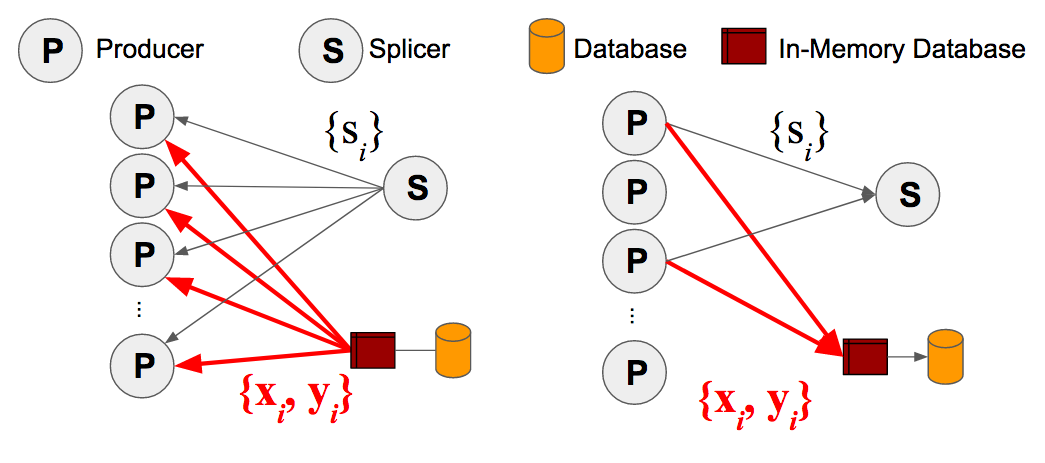
\includegraphics[width=19pc,angle=0]{figures/arch-parsplice.png}\\
  \caption{ParSplice is a ready-heavy HPC application where producers use a
  database for consistency. Replacing the single-node database with HXHIM
  improves performance with load balancing.
  \label{fig:arch-parsplice}}
\end{figure}


ParSplice~\cite{perez:jctc20150parsplice} is a molecular dynamics simulation
developed at LANL. It has 4 phases, as depicted in Figure~\ref{fig:arch-parsplice}:

\begin{enumerate}

  \item splicer (S) tells producers (P) to compute segments for state \(s_i\)

  \item P`s pull initial coordinates \{\(x_i, y_i\)\} from database

  \item a P inserts completed coordinates for segment \(s_i\) into database and
  S broadcasts next segment(s) \(s_j\) 

  \item P`s pull new segment coordinates \{\(x_j, y_j\)\}

\end{enumerate}

The database is single node (LevelDB or BerkeleyDB) with caches in front. Our
goal is to replace this architecture with a distributed key-value store to
solve the immediate sync problems that the ParSplice team is facting. Sliding
in something like MDHIM~\cite{greenberg:hotstorage2015-mdhim} has the added
benefit of enabling load balancing. ParSplice has distinct workload phases and
a well-known keyspace (Figure~\ref{fig:methodology-keyspace}) so its
performance should improve with better load balancing.

\subsection{MDHIM: Key-Value Store for HPC}
\label{sec:hxhim}

\begin{figure}[tb]
  \noindent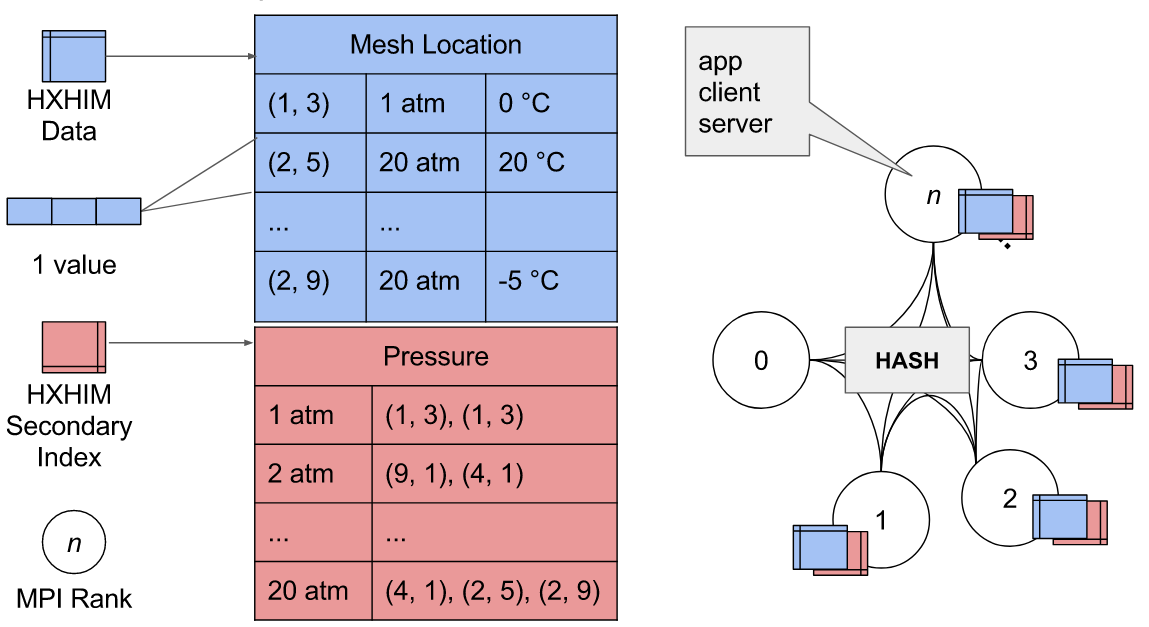
\includegraphics[width=19pc,angle=0]{figures/arch-hxhim.png}\\
  \caption{The MDHIM architecture.}
  \label{fig:arch-hxhim}
\end{figure}

% What is MDHIM
MDHIM is a key-value store designed for HPC architectures and multi-dimensional
data. It is based off MDHIM~\cite{greenberg:hotstorage2015-mdhim}, the
multi-dimensional indexing middleware. Figure~\ref{fig:arch-hxhim} has a crude
sketch of the MDHIM architecture. Each MPI rank has an instance of the
application, which has the client library linked in. An MPI rank can also have
a ``range server", which stores the key-value pairs in a local databse (either
LevelDB or MySQL). Data is located with a consistent hash, which is
configurable.

% What are the indexes?
The primary and secondary indices shown on the right side of
Figure~\ref{fig:arch-hxhim} are views of the data that the range server
manages.  The primary index is the same hash used by the global partitioner.
The secondary index or indices are user-defined tables organized in a different
way from the primary index. The goal of the secondary indices is to speed up
queries that need to aggregate dat ({\it e.g.} find the maximum values). In the
example, the range server and the key in the primary index is located with a
hash of the mesh location. The secondary index is organized by pressure, so
queries asking for a certain atmosphere can be serviced in O\(1\), consisting
of one lookup in the pressure index and one lookup into the primary index.

% Why is it tailored to HPC?
MDHIM tailors its mechanisms and policies to HPC, showing improved performance
over cloud-based key-value stores like Cassandra. It has cursor types for
walking the key-value store, bulk operations for exploiting data locality,
per-job server spawning, and pluggable backends for its local database and
network type (infiniband/RDMA). Its policies are flexible, supporting
customized partitioning strategies and user-defined secondary indices. This
allows the system to choose whether to send load to the client or server.

%\subsection{Comparing Mantle and MDHIM}
%\begin{table*}
%\centering
%\begin{tabular}[tb]{ r | l | l | l | l }
%                       & 
%                       & \multicolumn{1}{c|}{\centering Both} 
%                       & \multicolumn{1}{c|}{\centering Mantle/CephFS}
%                       & \multicolumn{1}{c}{\centering MDHIM}
%                       \\\hline
%  workload   & characteristics     & small/frequent requests  & data access            & data management \\
%             & write-intensive     & partition across cluster & fragment directories*  & NOT IMPLEMENTED \\
%             & read-intensive      & replicate across cluster & copy directories*      & NOT IMPLEMENTED \\\hdashline
%  system     & measure workload    & yes                      & directory temperature  & range server counts \\
%  mechanisms & measure utilization & yes                      & CPU, network, memory   & range server buffer size \\
%             & migrate resources   & almost                   & \texttt{export\_dir()} & \texttt{mdhimB}\{\texttt{Get}, \texttt{Put}\}\texttt{()} \\
%             & partition resources & yes                      & subtrees \& dirfrags   & secondary index, cursor type, bulk operations\\\hdashline
%  migration  & interval            & configurable             & every 10 seconds       & every query \\
%  decisions  & global state        & decentralized decisions  & heartbeats for metrics & NOT IMPLEMENTED \\
%  \multicolumn{5}{c}{}\\
%  \multicolumn{5}{c}{\tiny *Mechanisms implemented in CephFS, not integrated into Mantle}
%\end{tabular}
%\caption{Comparing the design goals and implementatons of Mantle and MDHIM.}
%\label{fig:arch-comparison}
%\end{table*}
%
%% Why are the designed for the same type of workload?
%The ``Both" column of Table~\ref{fig:arch-comparison} shows how Mantle and
%MDHIM have similar designs. The workloads are very similar as the the services
%respond to small and frequent requests, which results in hot spots and flash
%crowds. As a result, popularity of the data, not the size, drives distribution
%in both systems. Both workloads also have data locality so the systems have
%mechanisms for leveraging requests with similar semantic meaning.  Finally, the
%overall design of both systems is decentralized meaning that there is no
%centralized scheduler and each server has an inconsistent global view.
%
%% What are the challenges?
%Despite the similarities, integrating the Mantle API with MDHIM has both design
%and technical challenges. Mantle is reactive to the workload as opposed to
%MDHIM migrations, which are triggered based on the request type. As a result,
%Mantle has functionality for exchanging server utilization (CPU, network,
%memory) and workload (tracks request types). MDHIM 
%
%
%%This paper takes the API and load balancers designed in
%%Mantle~\cite{sevilla:sc15-mantle}, the programmabile file system metadata load
%%balancer for Ceph, and applies them to
%%MDHIM~\cite{greenberg:hotstorage2015-mdhim}, the distributed key-value store
%%designed for HPC.
%
%
%
%Results should show, In order from most likely to least likely:
%
%\begin{enumerate}
%
%  \item HPC key-value store workloads are structured (because they are mostly
%  workflows and simulations) that their job phases can be learned and exploited
%  using dynamic load balancing policies.
%
%  \item HPC key-value store workloads are so structured that one
%  policy-fits-all
%
%  \item HPC key-value store workloads are not structured enough to be learned
%
%  \item HPC key-value store workload hotspots/flash crowds are too fast to be
%  exploited
%
%\end{enumerate}

\section{ParSplice Keyspace Analysis}
\label{sec:parsplice-keyspace-analysis}
%IT HAS 8K keys!  How did we take these measurements

We instrumented ParSplice with performance counters and keyspace counters.  The
performance counters track ParSplice activities while keyspace counters track
which keys were being accessed by the ParSplice ranks. Because the keyspace
counters have high overhead we only turn them on for the keyspace analysis.

The cache hierarchy was unmodified but for the back-end persistent database, we
replaced BerkeleyDB on NFS with LevelDB on Lustre. Original ParSplice
experiments showed that BerkeleyDB's syncs caused reads/writes to bottleneck on
the persistent database node. We also use Riak's customized
LevelDB\footnote{https://github.com/basho/leveldb} version, which comes
instrumented with its own set of performance counters.

\subsection*{Testbed: Cray XC40}

All experiments ran on Trinitite, a Cray XC40 with 100 nodes each with 32 Intel
Haswell 2.3GHz cores.  Each node has 128GB of RAM and our goal is to limit the
size of the database to 3\% of RAM. Note that this is an addition to the 30GB
that ParSplice uses to manage other ranks on the same node.  A single Cray node
produced trajectories that are \(5\times)\) longer than our 10 node CloudLab
clusters and \(25\times\) longer than our in-house 10 node cluster. As a
result, it reaches different job phases faster and gives us a more
comprehensive view of the workload. The performance gains compared to the
commodity clusters has more to do with memory/PCI bandwidth than network.

\begin{figure}[t]
  \noindent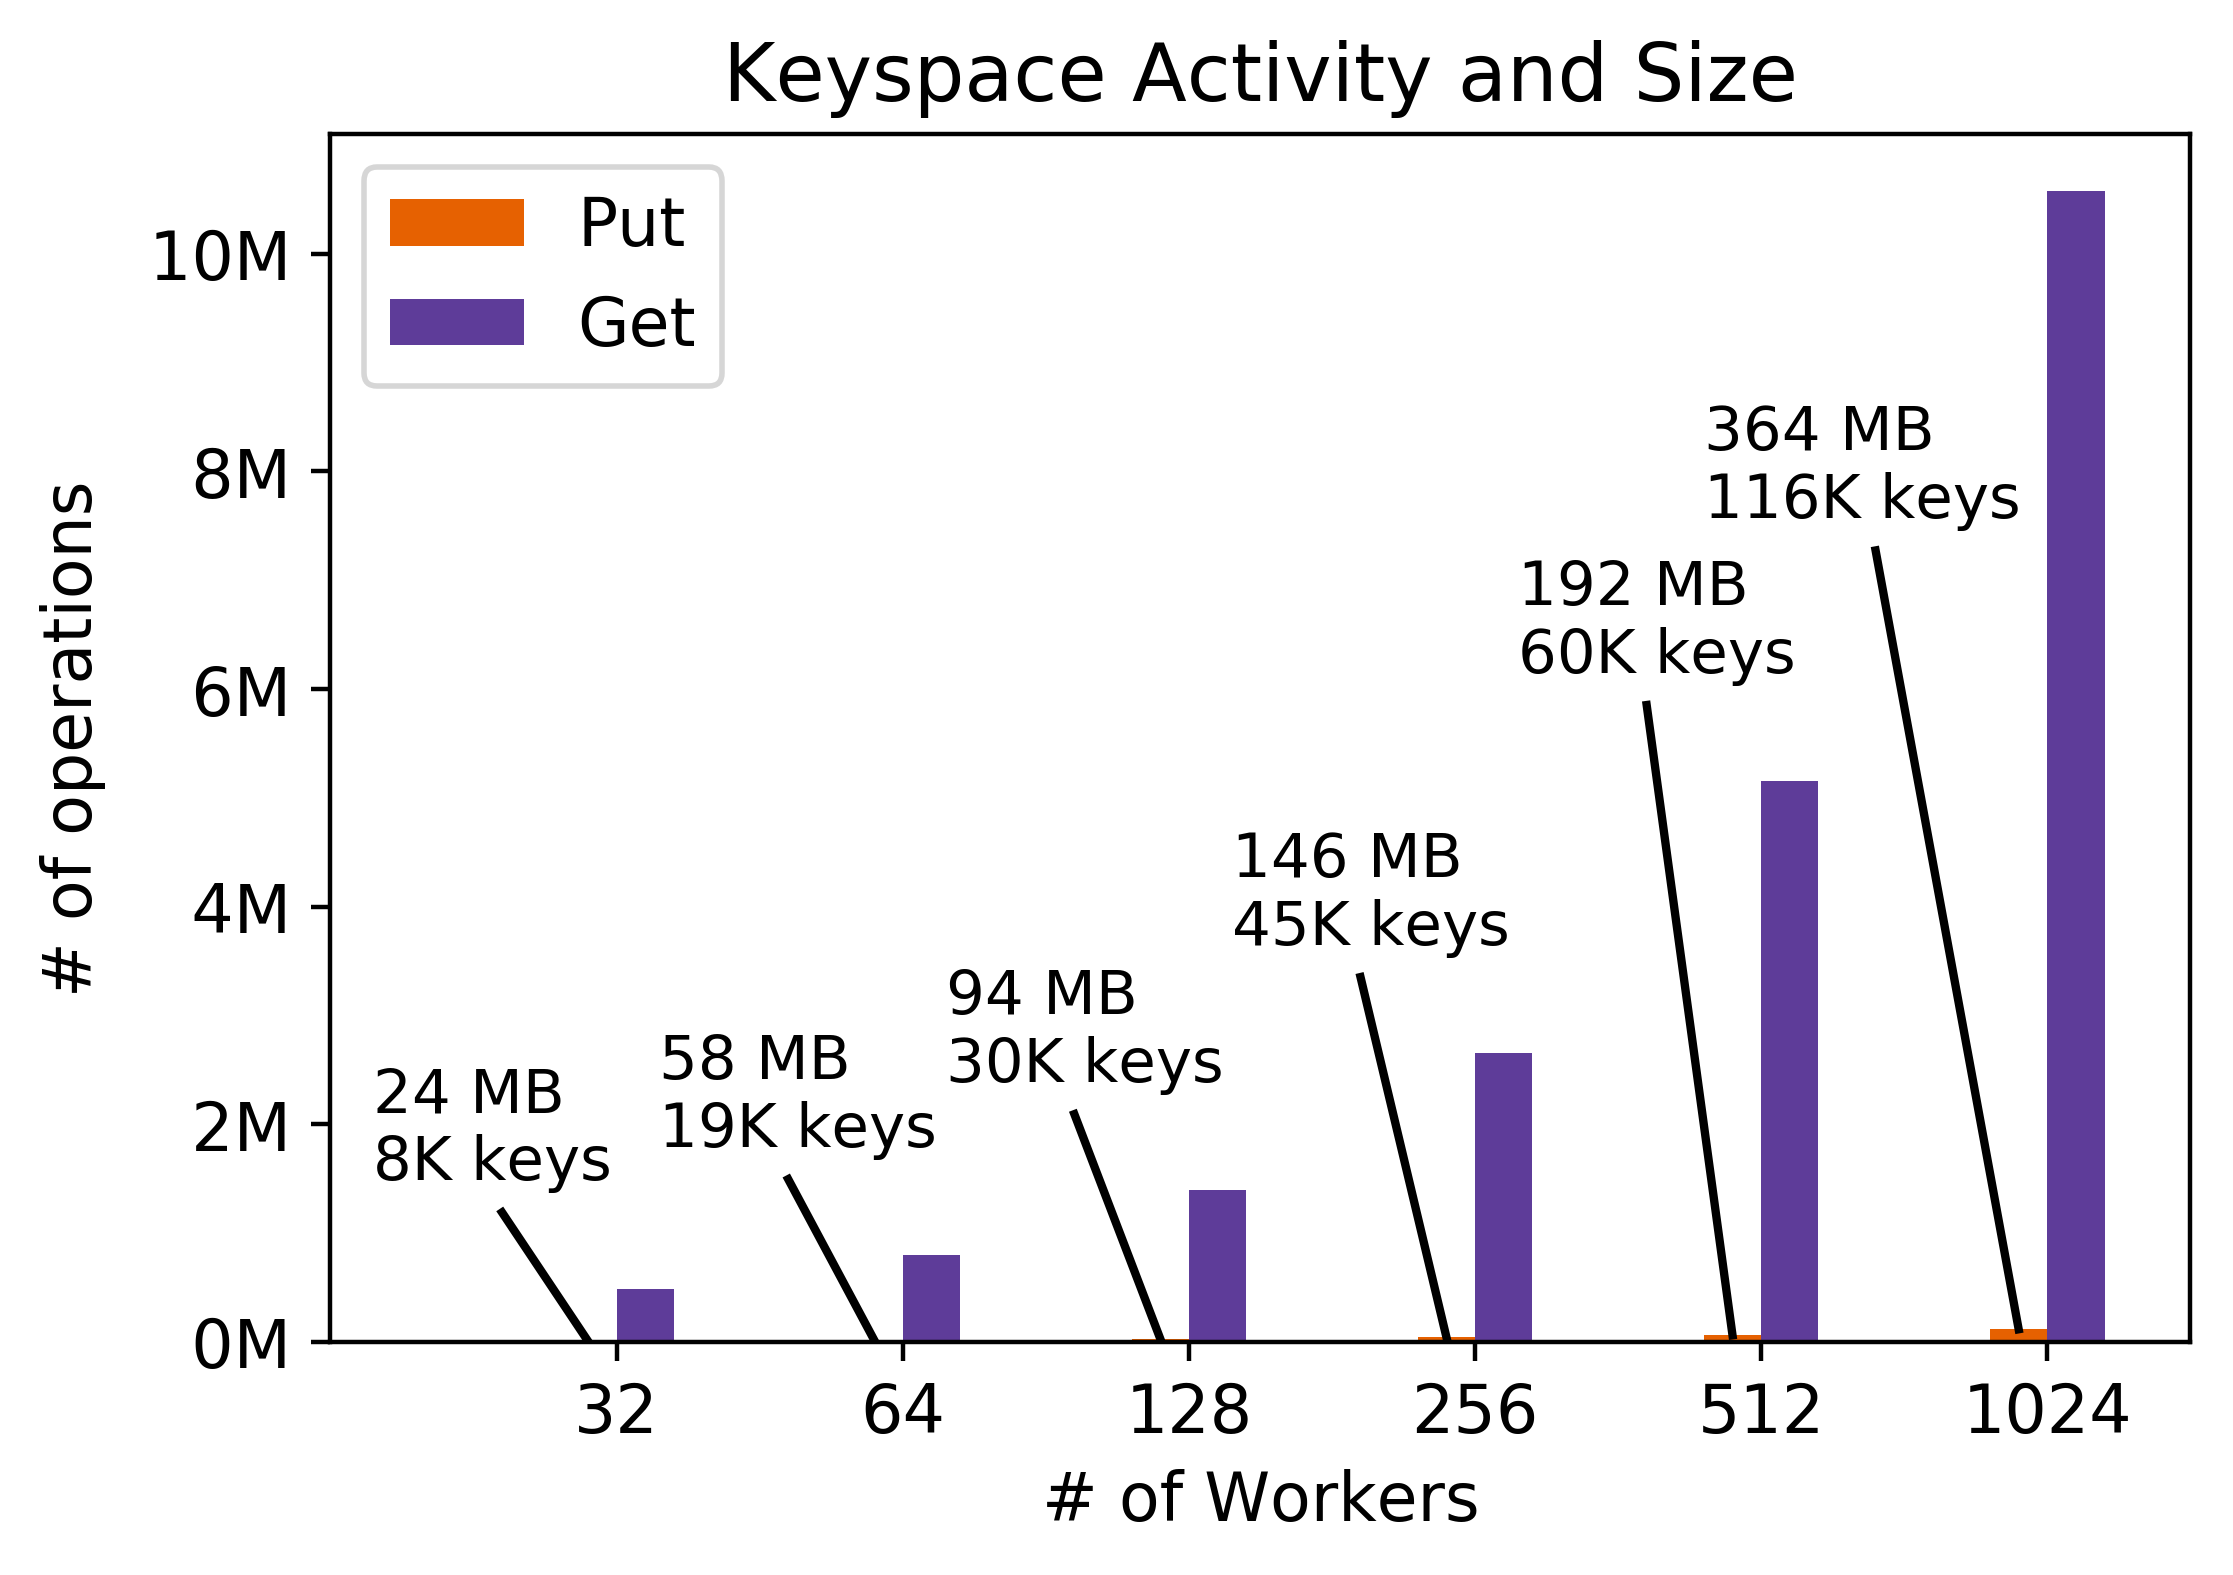
\includegraphics[width=0.4\textwidth]{figures/methodology-keyspace.png}\\
  \caption{The keyspace size is small but must satisfy many reads as workers
  calculate new segments. Based on these trends, it is likely that we will need
  more than one node to manage segment coordinates when we scale the system or jobs up.
  \label{fig:methodology-keyspace}}
\end{figure}

\begin{figure}[t]
  \noindent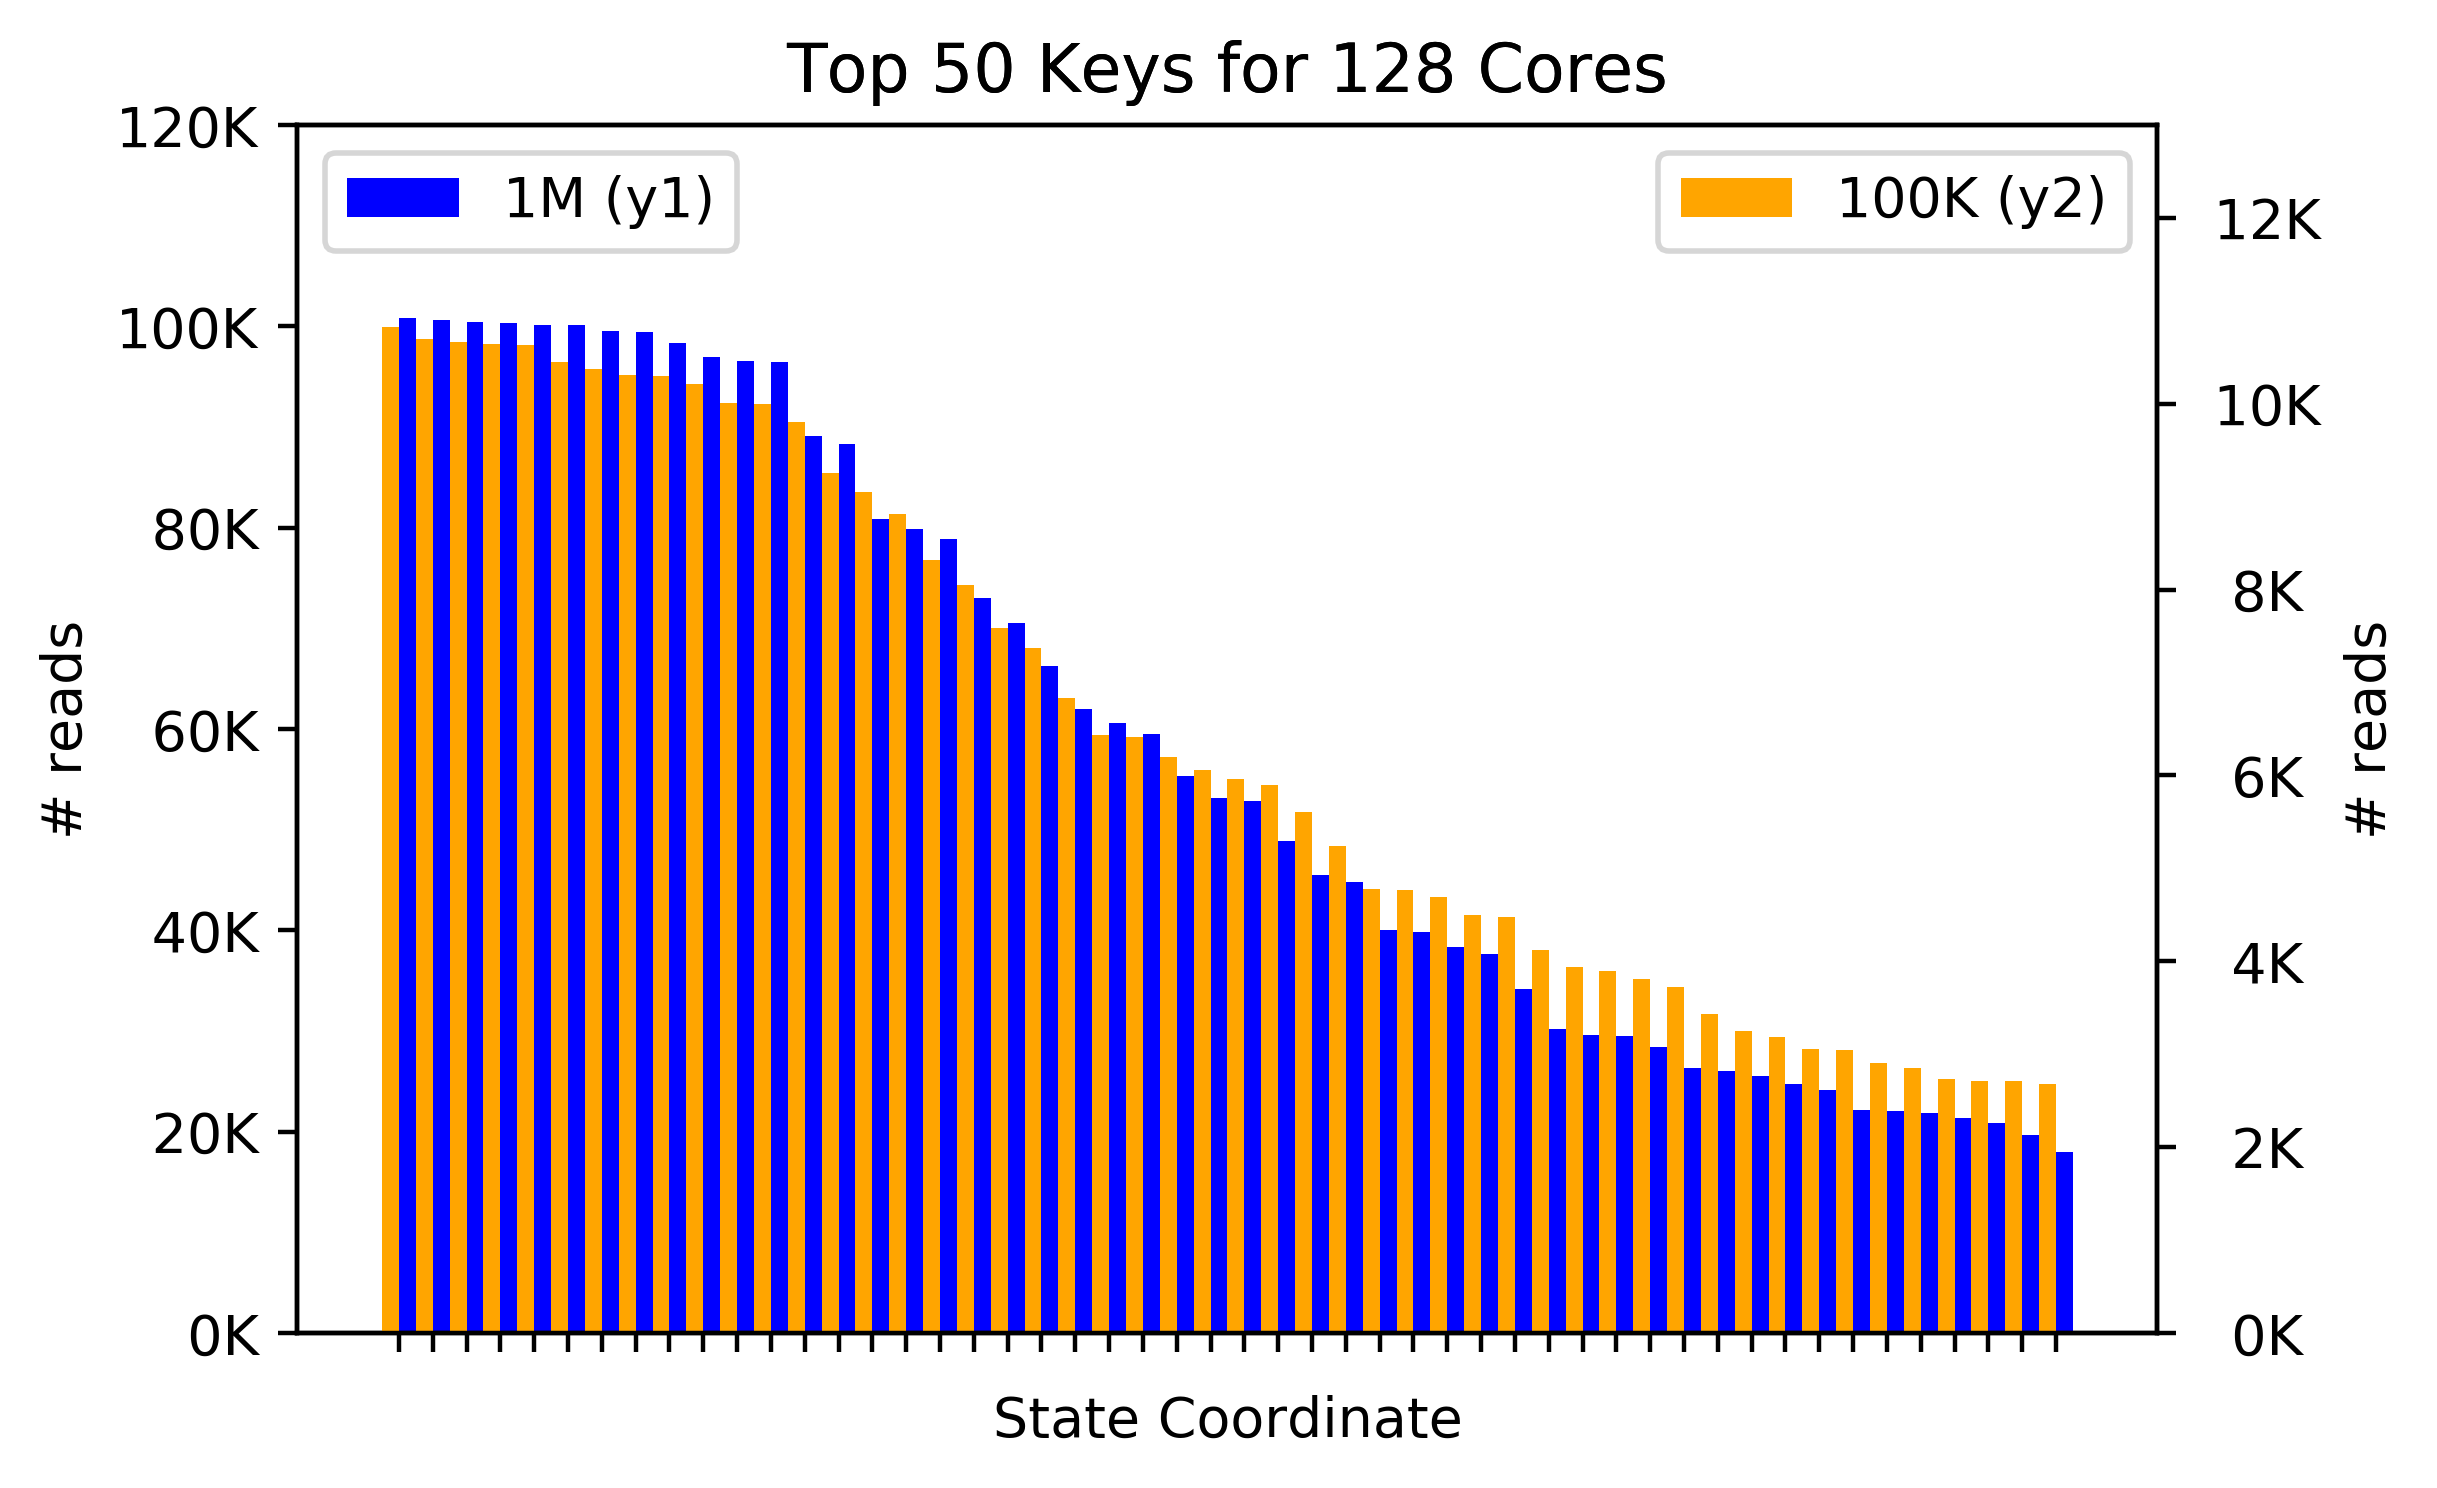
\includegraphics[width=0.4\textwidth]{figures/methodology-keys.png}\\
  \caption{The keyspace imbalance is due to workers generating deep
  trajectories and reading the same coordinates. Over time, the accesses get
  dispersed across different coordinates resulting in some keys being more
  popular than others.\label{fig:methodology-keys}}
\end{figure}

\subsubsection*{Scalability concerns} 
Figure~\ref{fig:methodology-keyspace} shows the keyspace size (black
annotations) and request load (bars) after a one hour run with a different
number of workers (\(x\) axis). While the keyspace size and capacity is
relatively modest the trends are concerning: memory usage scales with the
number of workers and Trinitite has 6000 cores. Furthermore, the size of the
keyspace scales with the length of the run. Extrapolating these magnitudes puts
an 8 hour run across all 100 Trinitite nodes at 20GB for the cache, which, in
addition to the 30GB base memory that ParSplice uses, puts the memory usage far
above the 4\% threshold we set earlier.

\subsubsection*{An active but small keyspace} 
The bars show \(50-100\times\) as many reads (\texttt{get()}) as writes
(\texttt{put()}).  Worker tasks read the same key for extended periods because
the trajectory segment is stuck in a superbasin composed of local minima, so
many coordinates are needed before the trajectory moves on. Writes only occur
for the final state of segments generated by worker tasks; their magnitude is
smaller than reads because the caches ignore redundant write requests. The
number of read and write requests are highest at the beginning of the run when
worker tasks generate segments for the same state, which is cheap. This type of
keyspace encourages replication across a cluster.  

\subsubsection*{Entropy increases over time} The reads per second in
Figure~\ref{fig:futurework-regimes} show that the number of requests decreases
and the number of active keys increases over time. The resulting key access
imbalance for the two growth rates in Figure~\ref{fig:futurework-regimes} are
shown in Figure~\ref{fig:methodology-keys}, where reads are plotted for each
unique state (\(x\) axis). Keys are more popular than others (up to
\(5\times\)) because worker tasks start generating states with different
coordinates later in the run.

\subsubsection*{Entropy growth is structured} The access patterns reflect the
locality of computation: worker tasks stuck in state basins generate segments with
similar coordinates. The growth rate, temperature, and number of workers
changes that locality, which has an effect on the structure of the keyspace.
Figure~\ref{fig:methodology-keys} shows that the number of reads changes with
different growth rates, but that spatial locality is similar ({\it e.g.}, some
keys are still \(5\times\) more popular than others).
Figure~\ref{fig:futurework-regimes} shows how entropy for different growth
rates has temporal locality, as the reads per second for 1M looks like the
reads per second for 100K stretched out along the time axis.  Trends also exist
for temperature and number of workers but are omitted here for space. This
structure means that we can learn the regimes and adapt the storage system to
it. 

\section{Static Load Balancing}
\label{sec:static-load-balancing}

% technical details
In the original ParSplice implementation, each cache node as much memory as it
wants to store segment coordinates. We limit the size of the cache using an LRU
eviction policy, where the penalty for a cache miss is retrieving the data from
the persistent database.  We evict keys (if necessary) at every operation
instead of when segments complete because the cache fills up too quickly
otherwise and it reduces the overhead of key eviction.

% results: cache size trade-offs
\begin{figure}[t]
  \noindent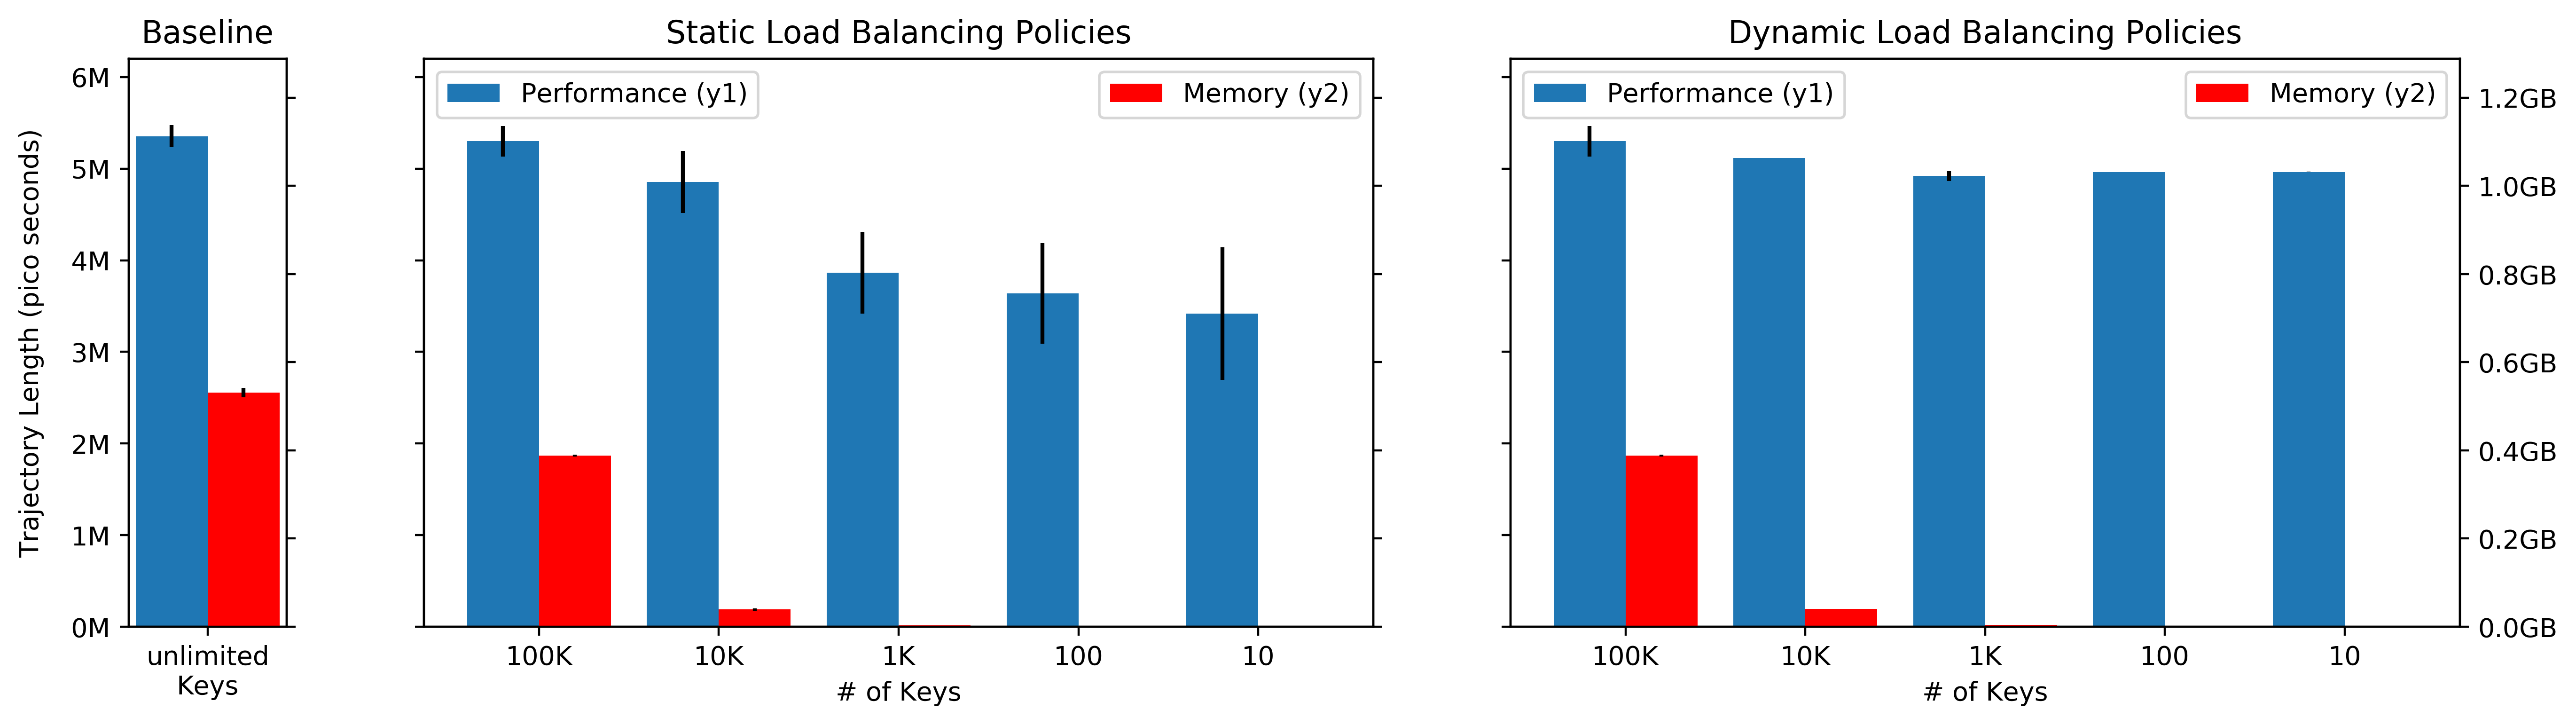
\includegraphics[width=0.4\textwidth]{figures/methodology-tradeoff.png}\\
  \caption{The performance and resource utilization trade-off for different
  cache sizes, which are enumerated along the \(x\) axis. ``Baseline" is
  ParSplice unmodified and the ``Static  Policies" limit the size of the
  cache to demonstrate the memory savings of smaller keyspaces on cache nodes.
  \label{fig:methodology-tradeoff}}
\end{figure}

The results for different cache sizes for a growth rate of 100K over a 2.5 hour
run is shown in Figure~\ref{fig:methodology-tradeoff}.  ``Baseline" is the
performance of unmodified ParSplice  measured in trajectory duration
(\(y\)-axis) and utilization is measured with memory footprint (\(y2\) axis) of
just the cache.  ``Static Load Balancing Policies" shares the \(y\)-axis and
shows the trade-off for different cache sizes. The error bars are the standard
deviation of 3 runs. 

% results: raw numbers
Although the keyspace grows to 150K, a 100K key cache achieves 99\% of the
performance. Decreasing the cache degrades performance and predictability.
While this result is not unexpected, it nonetheless achieves our goal of
showing the benefits of load balancing keys across nodes and that smaller
caches on each node are an effective way to save memory without completely
sacrificing performance.

\section{The Need for Dynamic Load Balancing Policies}
\label{sec:the-need-for-dynamic-load-balancing-policies}

% why is the performance lower for smaller caches?
Despite the memory savings, our results suggest that dynamic load balancing
policies could save even more memory.  Figure~\ref{fig:methodology-tradeoff}
show that a 100K key cache is sufficient as a static policy but the top graph
in Figure~\ref{fig:motivation-regimes} indicates that the cache size could be
much smaller. That graph shows that the beginning of the run is characterized
by many reads to a small set of keys and the end sees much lower reads per
second to a larger keyspace. Specifically, it shows only about 100 keys as
active in the latter half of the run.

After analyzing traces, we see that the 100 key cache is insufficient because
the persistent database cannot service the read-write traffic.  According to
Figure~\ref{fig:motivation-regimes}, the read requests arrive at 750 reads per
second in addition to the writes that land in each tier (about 300 puts/second,
some redundant). This traffic triggers a LevelDB compaction and reads block,
resulting in very slow progress.  Traces verify this hypothesis and show reads
getting backed up as the read/write ratio increases. To recap, small caches
incur too much load on the persistent database  at the beginning of the run but
should suffice after the initial read flash crowd passes because
the keyspace is far less active. This suggests a two-part load balancing
policy.

% what is mantle
To explore dynamic load balancing policies ({\it i.e.} policies that change
during the run), we use the Mantle approach.  Mantle is a framework built on the
Ceph file system that lets administrators control file system metadata load
balancing policies. The basic premise is that load balancing policies can be
expressed with a simple API consisting of ``when", ``where", and ``how much".
The succinctness of the API lets users inject multiple, dynamic policies.

% Why is this a good idea
Although ParSplice does not use a distributed file system, its workload is very
similar because the minima key-value store responds to small and frequent
requests, which results in hot spots and flash crowds.  Modern distributed file
systems have found efficient ways to measure, migrate, and partition metadata
load and have shown large performance gains and
better scalability~\cite{zheng:pdsw2014-batchfs, zheng:pdsw2015-deltafs,
grider:pdsw2015-marfs, ren:sc2014-indexfs, patil:fast2011-giga+,
brandt:msst2003-lh}.  Previous work quantified the speedups achieved with
Mantle and formalized balancers that were good for file systems.

\begin{figure}[t]
  \noindent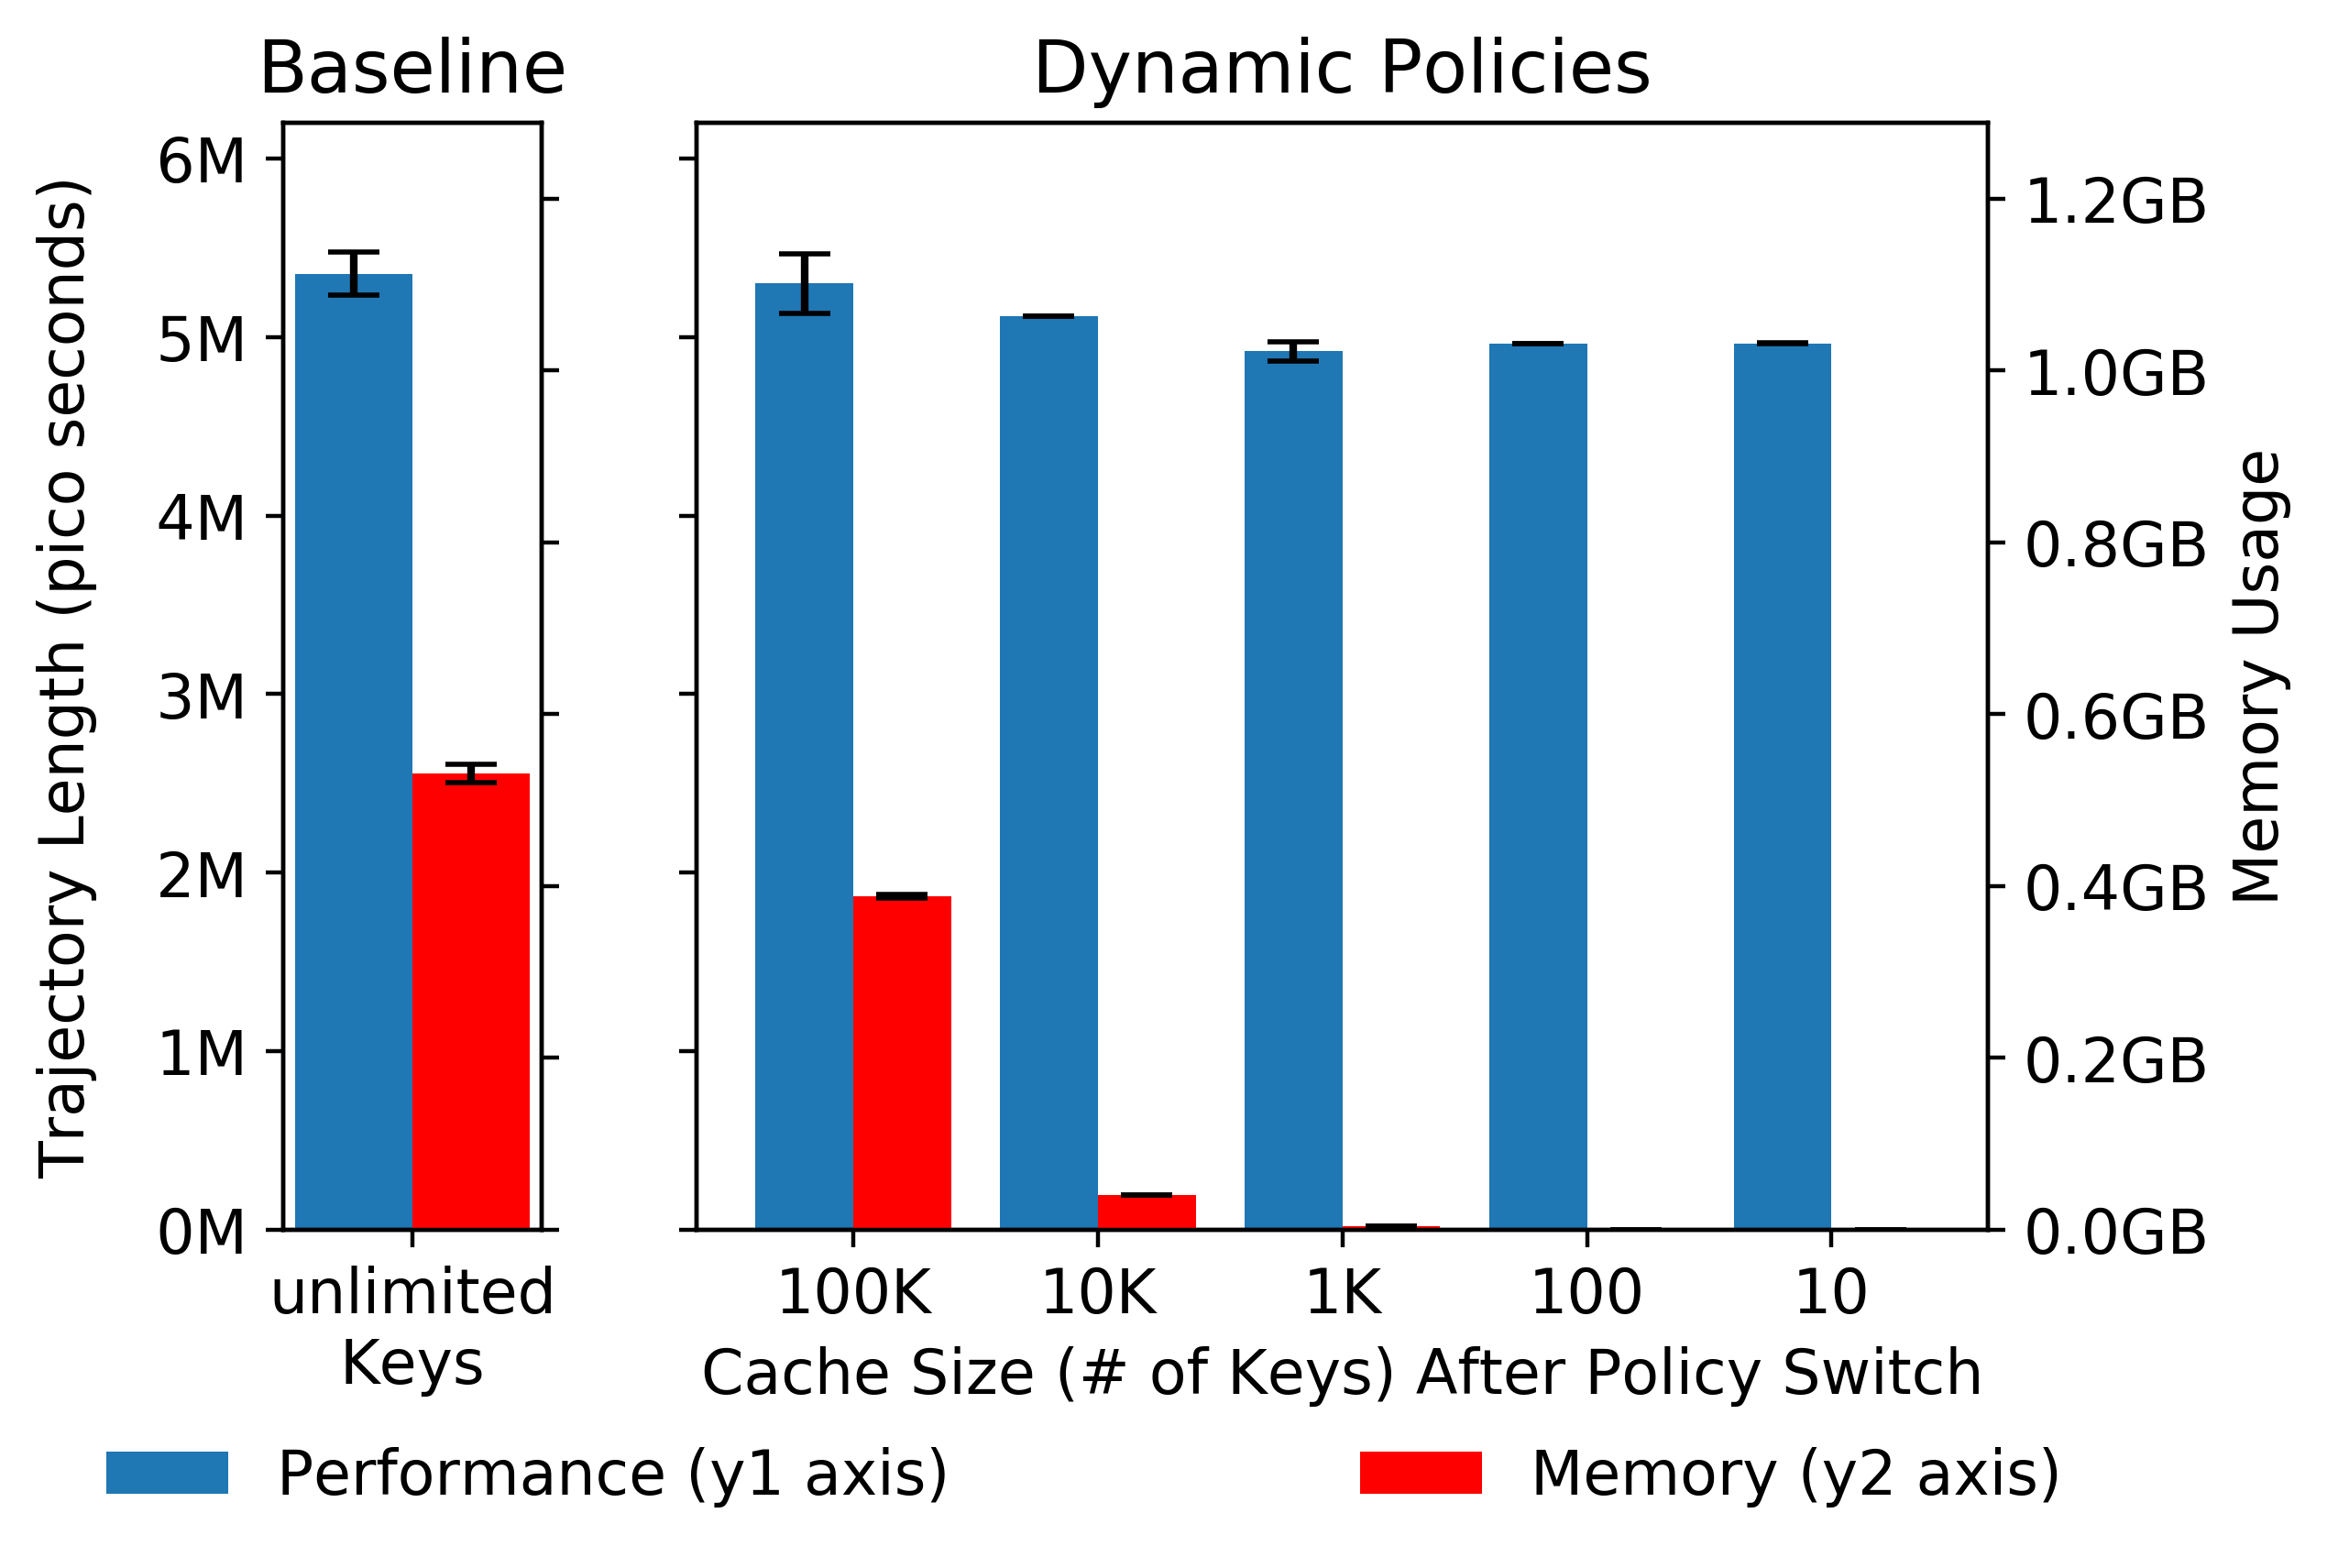
\includegraphics[height=5cm,width=0.5\textwidth]{figures/methodology-tradeoff-dynamic.png}\\
  \caption{The performance and resource utilization trade-off of using a
  dynamic load balancing policy that switches to a constrained cache policy after absorbing
  the initial burstiness of the workload. The sizes of these smaller caches are
  on the \(x\) axis.  \label{fig:methodology-tradeoff-dynamic}}
\end{figure}

Figure~\ref{fig:methodology-tradeoff-dynamic} shows the results of using the
Mantle API to program a dynamic load balancing policy into ParSplice that
switches between two policies:

\begin{itemize}
  \item unlimited growth policy: cache increases on every write
  \item \(n\) key limit policy: cache constrained to \(n\) keys
\end{itemize}

We trigger the policy switch at 100K keys to absorb the flash crowd at the
beginning of the run. Once triggered, keys are evicted to bring the size of the
cache down to the threshold.  In the bar chart, the cache sizes for the \(n\)
key limit policy are along the \(x\) axis.

% results: same level of performance can be achieved 
The dynamic policies show better performance than the single \(n\) key
policies. The performance and memory utilization for a 100K key cache size is
the same as the 100K bar in Figure~\ref{fig:methodology-tradeoff-dynamic} but
the rest reduce the size of the keyspace after the read flash crowd.  We see
the worst performance when the engine switches to the 10 key limit policy,
which achieves 94\% of the performance while only using 40KB of memory. 

% caveats: it is calculating 90% of the trajectory, memory value reported is final
\subsubsection*{Caveats}

The results in Figure~\ref{fig:methodology-tradeoff-dynamic} are slightly
deceiving for three reason: (1) segments take longer to generate later in the
run, (2) the memory footprint is the value at the end of 2.5 hours, and (3)
this policy only works well for the 2.5 hour run.  For (1), the curving down of
the simulation vs. wall-clock time is shown in
Figure~\ref{fig:methodology-trajectory}; as the nanoparticle grows it takes
longer to generate segments so by the time we reach 2 hours, over 90\% of the
trajectory is already generated.  For (2), the memory footprint is around 0.4GB
until we reach 100K key switch threshold. In
Figures~\ref{fig:methodology-tradeoff}
and~\ref{fig:methodology-tradeoff-dynamic} we plot the final value. For (3),
Figure~\ref{fig:methodology-trajectory} shows that the cache fills up with 100K
keys at time 7200 seconds and its size is reduced to the size listed in the
legend.  The curves stay close to ``Unlimited" for up to an hour after the
cache is reduced but eventually flatten out as the persistent database gets
overloaded. 10K and 100K follow the ``Unlimited" curve the longest and are
sufficient policies for the 2.5 hour runs but anything longer would need a
different dynamic load balancing policy.

\begin{figure}[t]
  \noindent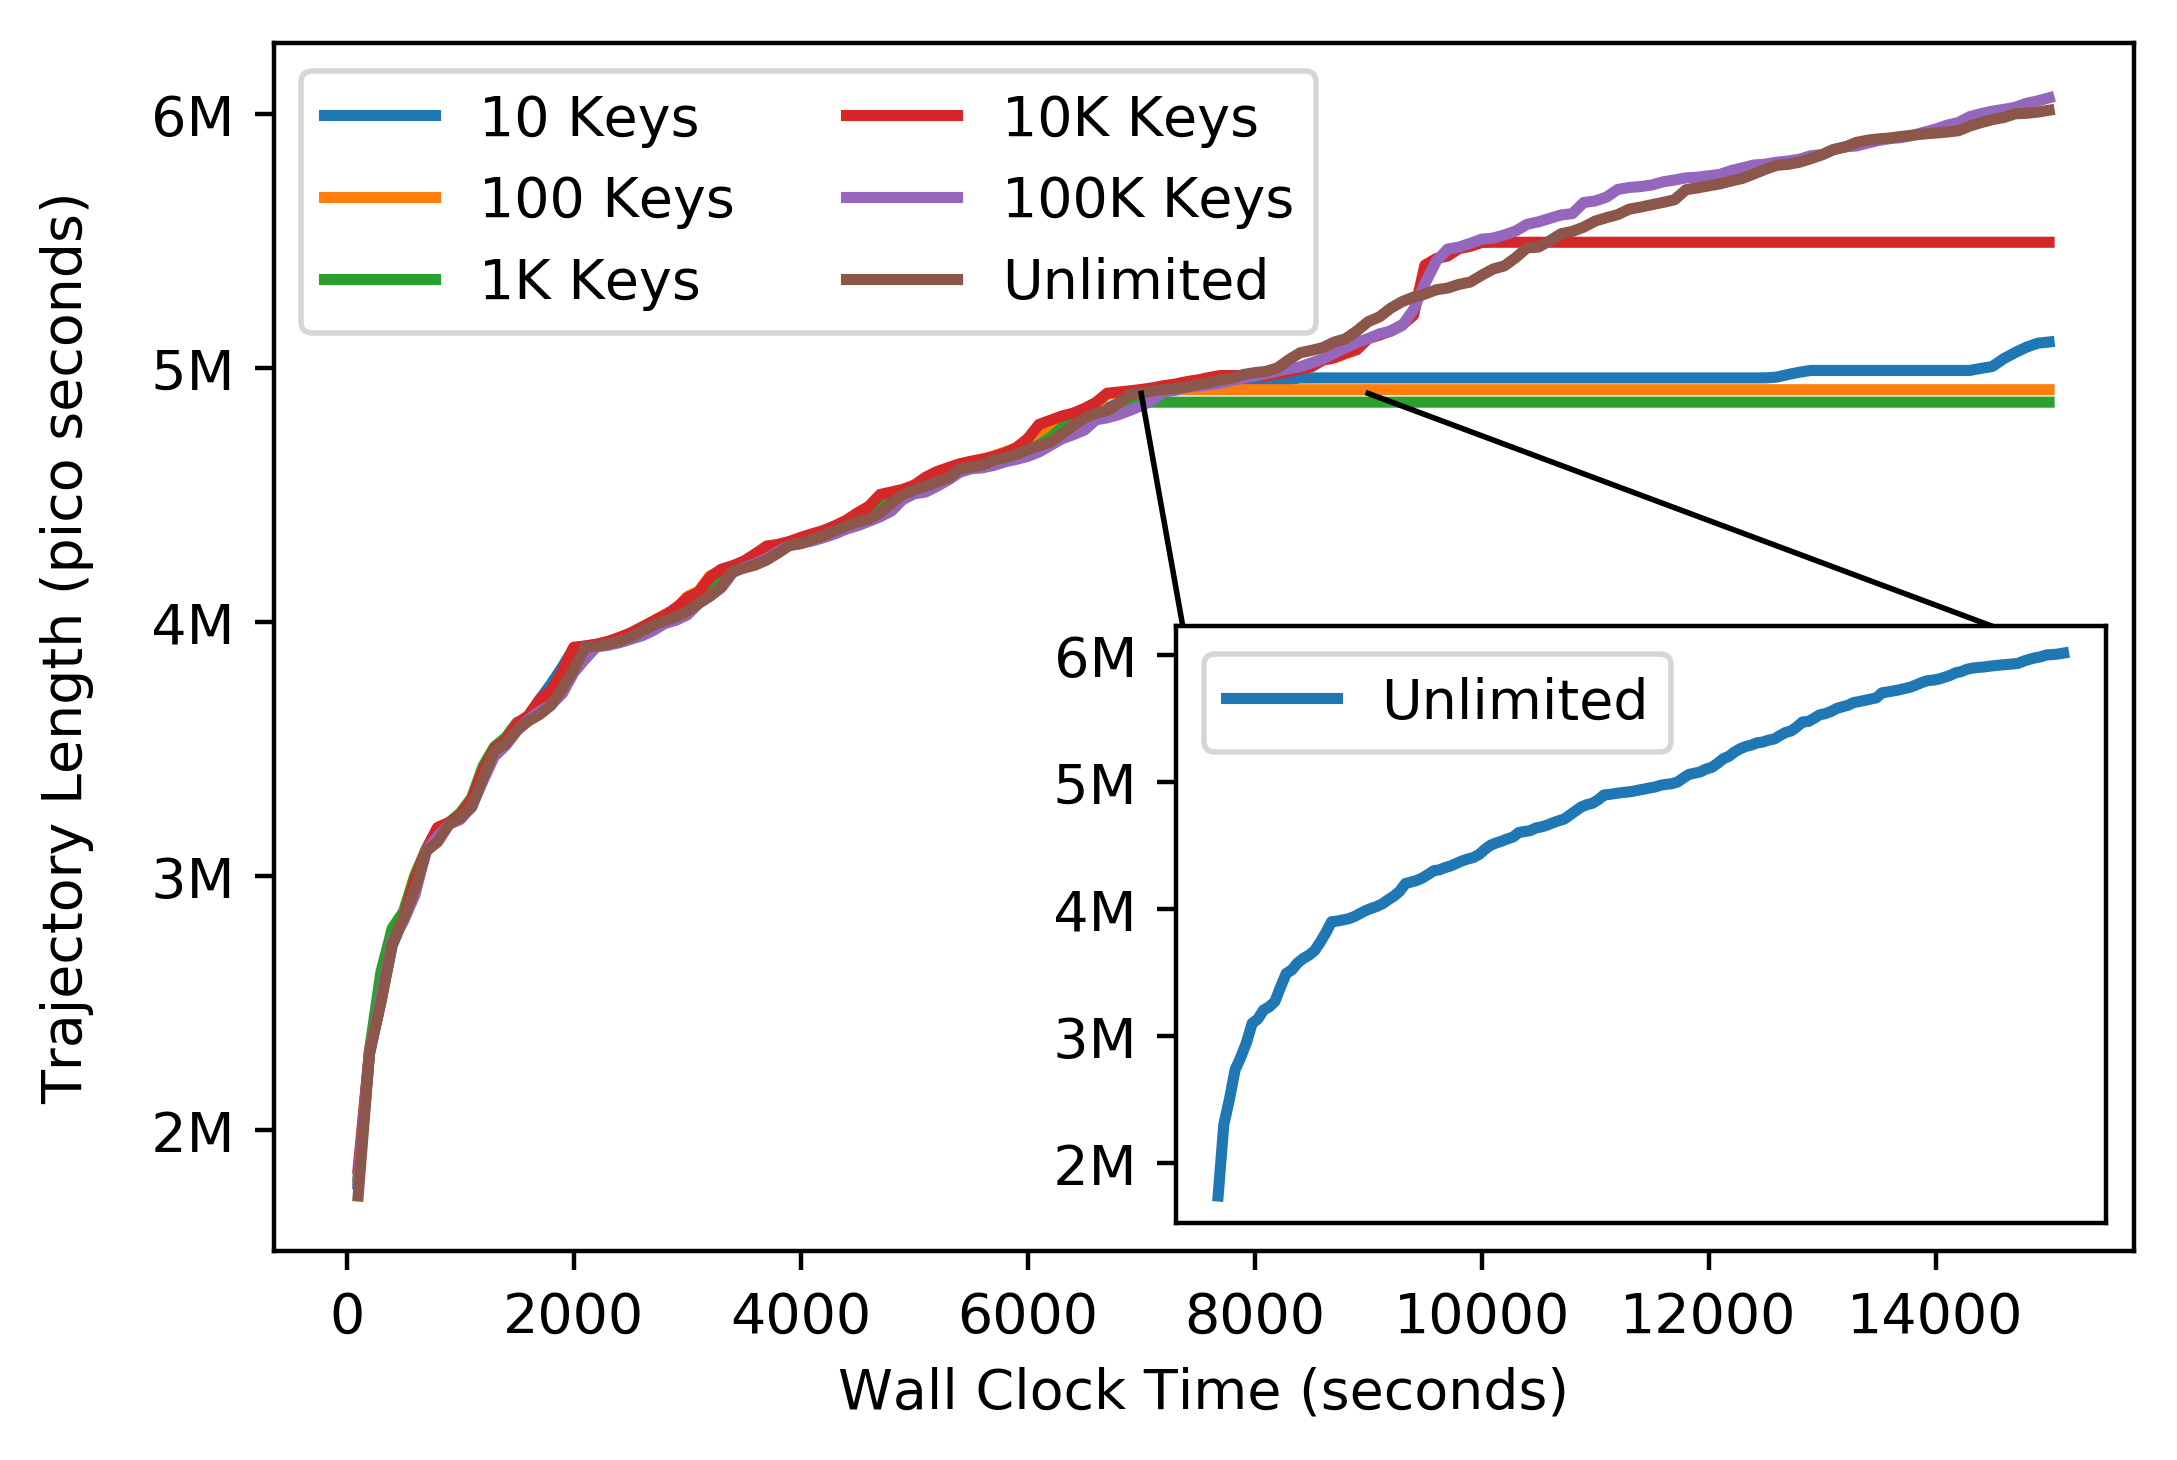
\includegraphics[height=5cm,width=0.4\textwidth]{figures/methodology-trajectory.png}\\
  \caption{The rate that the trajectory is computed decays over time (which is
  expected) but this skews the performance improvements in
  Figure~\ref{fig:methodology-tradeoff-dynamic}. Our dynamic policy works for 2.5
  hour jobs but not for 4 hour jobs.  \label{fig:methodology-trajectory}}
\end{figure}

% but the result is still valid
Despite these caveats, the result is still valid: we found a dynamic load
balancing policy that absorbs the cost of a high read throughput on a small
keyspace and reduces the memory pressure for a 2.5 hour run. Our experiments
show the effectiveness of the load balancing policy engine we integrated into
ParSplice, not that we were able to identify the best policy for all system
setups ({\it i.e.} different ParSplice parameters, number of worker tasks, and
job lengths).  To solve that problem, we need a way to identify what thresholds
we should use for different job permutations.



\section{Using ML for the Keyspace}
\label{sec:ml-for-the-keyspace}

We proved in the previous section that an optimal policy, based on the read
burstiness at the beginning of the run,  exists for a 100K growth rate on 8
nodes, but we cannot re-do this analysis for every workload, system, and
parameter permutation.  Fortunately,
Section~\S\ref{sec:parsplice-keyspace-analysis} shows that the keyspace size
and activity is structured. Rather than finding policies by hand again for
every cluster size, growth rate, and temperature, in this section we use
machine learning to inform the Mantle policy engine.  Machine learning is good
at two things: handling large design spaces and matching patterns. Our keyspace
analysis in Section~\ref{sec:parsplice-keyspace-analysis} demonstrated a large
design space and Figure~\ref{fig:motivation-regimes} shows 4 workload regimes:
one plateau of redundant reads at the beginning, decreasing requests per
second, and then two plateaus of steady requests per second. We start with a
simple clustering algorithm to attack this multi-dimensional design space
problem and detect workload regimes.

% implementation: 
We feed the read request rate from the 100K and 1M runs in
Figure~\ref{fig:motivation-regimes} into the K-means clustering algorithm as
(timestamp, ops/second) tuples\footnote{Note that the magnitudes are different
because Figure~\ref{fig:motivation-regimes} was run with keyspace tracing on,
which reduces performance}. We weight the timestamp and ops/second equally and
set the number of clusters to be 4.  We chose this initial K  based on visual
inspection of Figure~\ref{fig:motivation-regimes} Knowing that the setup
parameters transform the request rates temporally or spatially, this same
initial K should work for all setups. Once the algorithm identifies the
workload regimes, we select the start of the third regime as the point to
switch to a fixed sized cache because the request rate has lowered to
sustainable levels for the persistent database.

We plot throughput over time in Figure~\ref{fig:futurework-regimes} and
color each point with its assigned group. The black stars are the centroids,
also known as the center of K-means groups.  We run the algorithm for a variety
of request rate traces but only show the setups from
Figure~\ref{fig:motivation-regimes}. We also annotate the graphs with the
suggested cache size, which is calculated by looking up the timestamp for the
third regime that corresponds to the keyspace size in our performance counters.

% results: 1. identifies 4 phases, 2. picks different timestamps for the third
% regime, suggests proper key values.
The algorithm properly identifies the 4 workload phases: the plateau of
redundant reads, the phase with a large decrease in request rate, and the two
plateaus of steady read requests. It also picks different timestamps for the
start of the third regime, which aligns with our keyspace analysis and our
assertion that the growth parameters affect how long it takes the workload to
reach a certain phase.  Finally, the algorithm picks reasonable values for the
key cache size. The 100K growth rate selects a 55K cache size, which is between
our benchmarked optimal threshold for the high watermark value chosen to
absorb the read burst (100K) and the lower cache size we limit the system to
after the initial burst (10K). This result both reaffirms the results from the
previous section and provides hope that we can avoid lengthy parameters sweeps
for ParSplice in the future.

\begin{figure}[t]
\noindent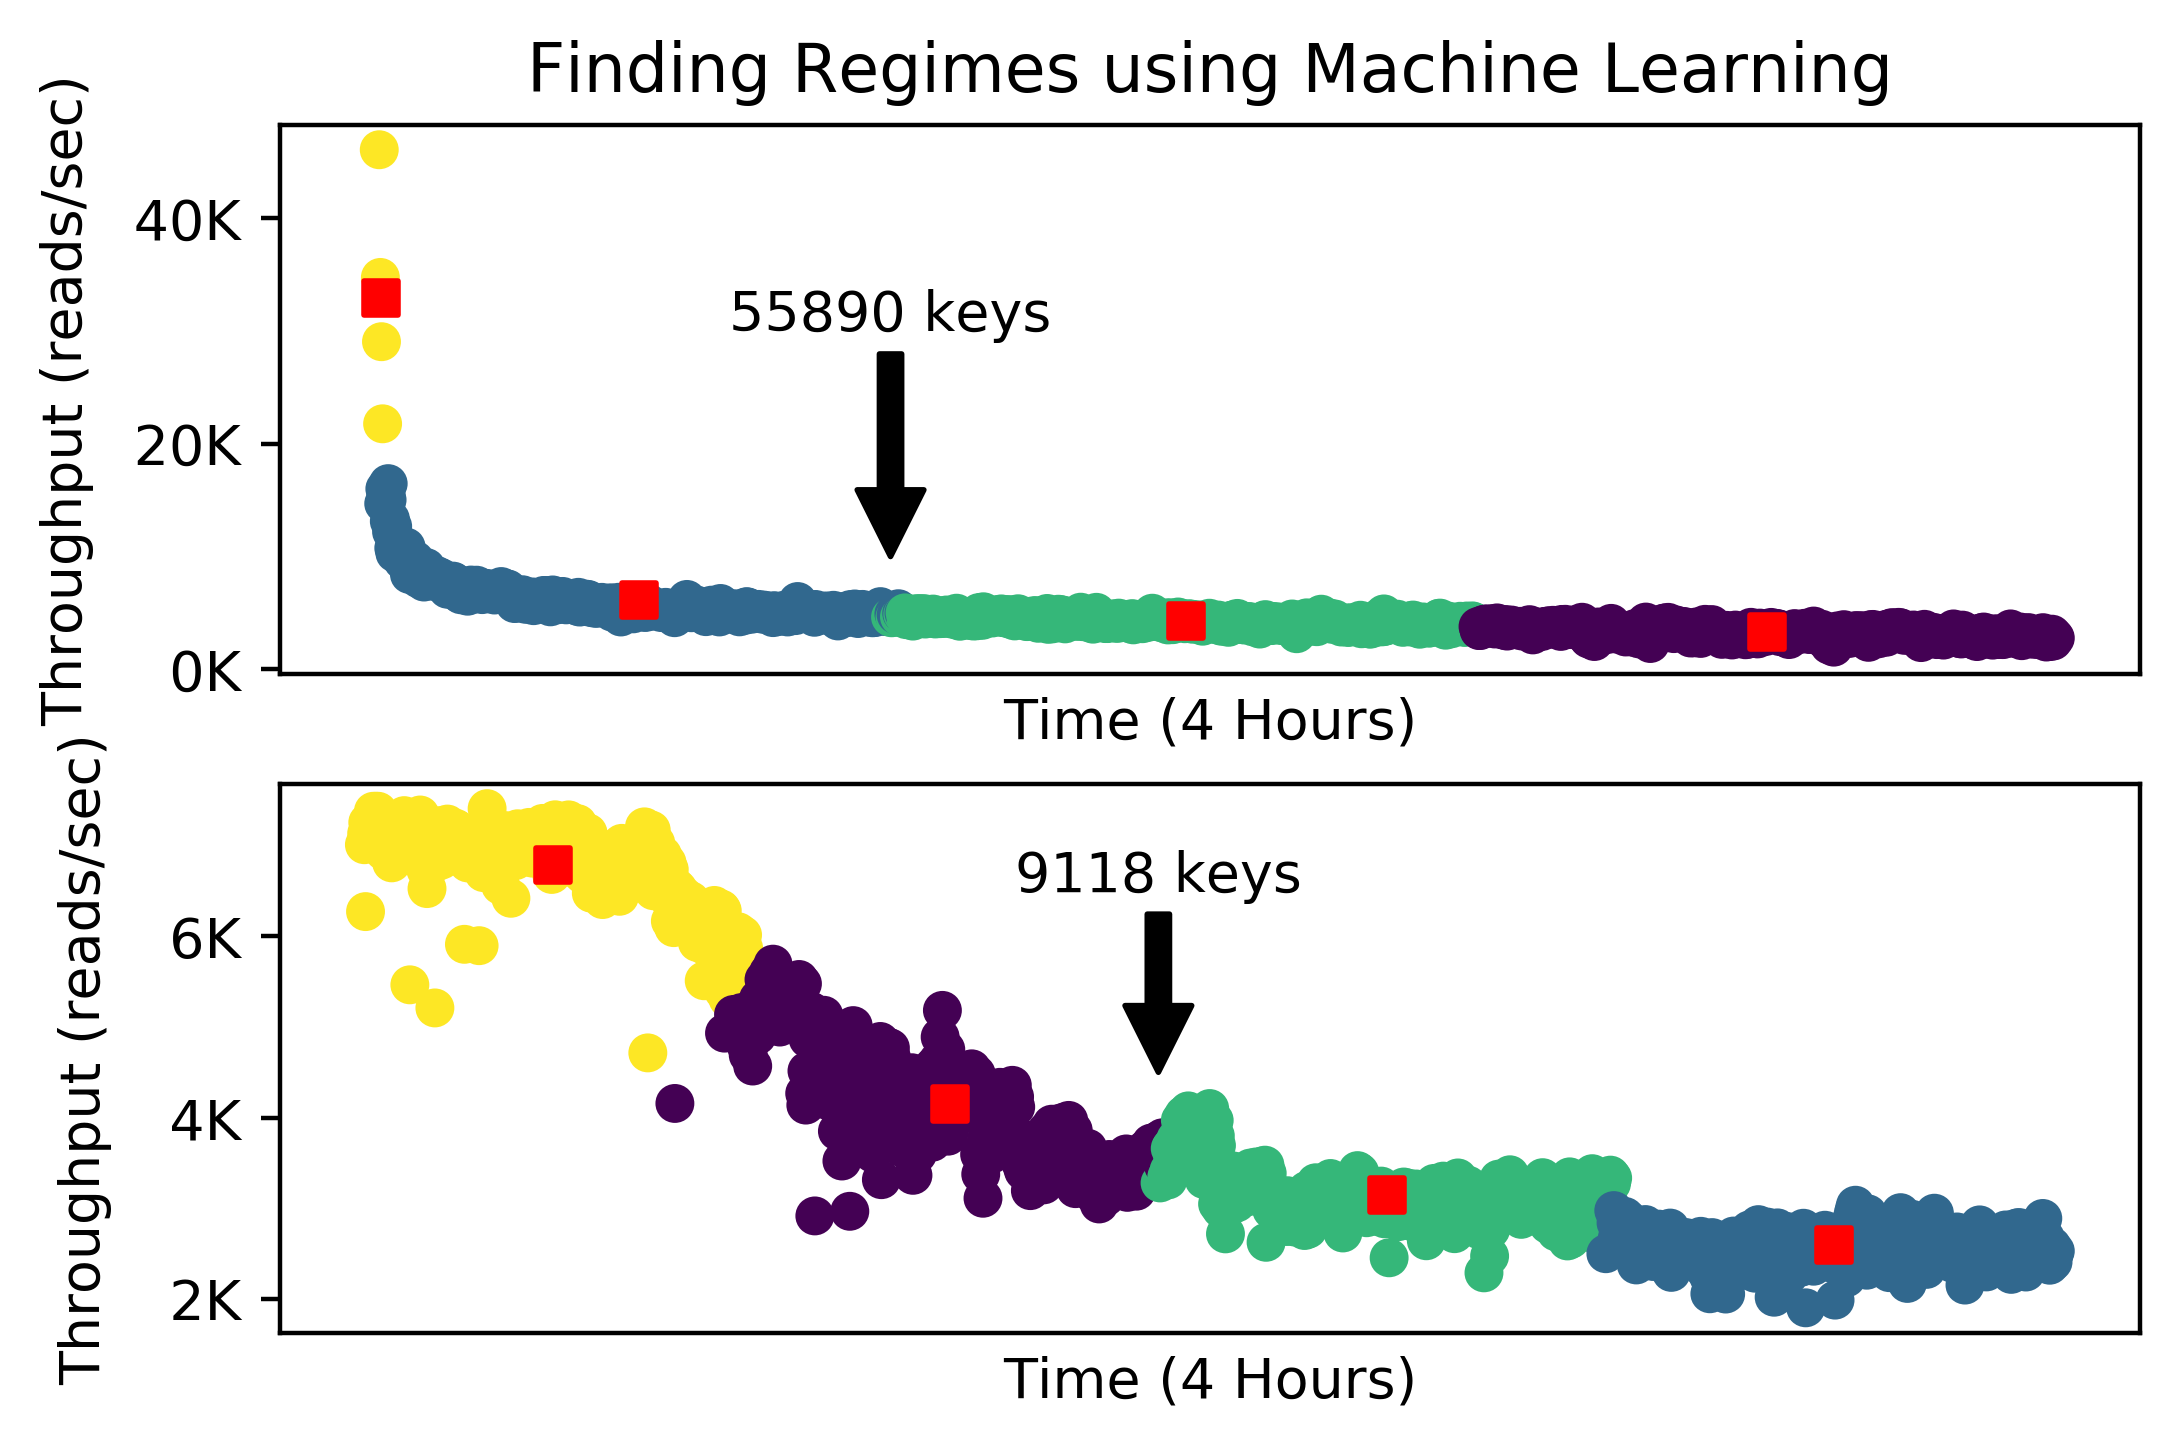
\includegraphics[width=0.4\textwidth]{figures/futurework-regimes.png}\\
  \caption{Learning the workload regimes with K-Means clustering helps pick
  keyspace size thresholds that can be fed into a dynamic load balancing policy
  engine, like Mantle. Specifying 4 clusters and selecting the third for
  informing the policy switch returns keyspace size thresholds similar to the
  values we found by hand in
  Section~\S\ref{sec:the-need-for-dynamic-load-balancing-policies}.
\label{fig:futurework-regimes}}
\end{figure}

\section{Related Work}

Key-value storage organizations for scientific applications is a field gaining
rapid interest. In particular, the analysis of the ParSplice keyspace and the
development of an appropriate scheme for load balancing is a direct response to
a case study for computation caching in scientific
applications~\cite{jenkins:ipdsw17-mochi}. In that work the authors motivated
the need for a flexible load balancing \emph{microservice} to efficiently scale
a memoization microservice. Our work is also heavily influenced by the
Malacology project~\cite{sevilla:eurosys17-malacology} which seeks to provide
fundamental services (e.g. write-ahead logging) at a much finer granularity
than has traditionally been performed with distributed file systems.  

\subsubsection*{File System Metadata}

State-of-the-art distributed file systems partition write-heavy workloads and
replicate read-heavy workloads.  IndexFS~\cite{ren:sc2014-indexfs} partitions
directories and clients write to different partitions by grabbing leases and
caching ancestor metadata for path traversal. ShardFS takes the replication
approach to the extreme by copying all directory state to all nodes. The Ceph
file system (CephFS)~\cite{weil:sc2004-dyn-metadata, weil:osdi2006-ceph} employs both
techniques to a lesser extent; directories can be replicated or sharded but the
caching and replication policies are controlled with tunable parameters.
Despite the obvious benefits of these protocols, these systems still need to be
tuned by hand with {\it ad-hoc} policies designed for specific applications. 

% policies
Setting policies for migrations is arguably more difficult than adding the
migration mechanisms themselves.  For example, IndexFS and CephFS use the
GIGA+~\cite{patil:fast2011-giga} technique for partitioning directories at a
predefined threshold. Mantle makes headway in this space by providing a
framework for exploring these policies, but does not attempt anything more
sophisticated (e.g., machine learning or autotuning) to create these policies. 

% ml and autotuning
\subsubsection*{Auto-tuning} Auto-tuning is a well-known technique used in
HPC~\cite{behzad:sc2013-autotuning, behzad:techreport2014-io-autotuning}, big
data systems systems~\cite{herodotou_starfish_2011}, and
databases~\cite{schnaitter_index_2009}.  Like our work, these systems focus on
the physical design of the storage ({\it e.g.} cache size) but since we focused
on a relatively small set of parameters (cache size, migration tresholds), we
did not need anything as sophisticated as the genetic algorithm used
in~\cite{behzad:sc2013-autotuning}.  We cannot drop these techniques into
ParSplice because the magnitude and speed of the workload hotspots/flash crowds
makes existing approaches less applicable. 

\subsubsection*{Distributed KV Stores}

Our goal is to use MDHIM~\cite{greenberg:hotstorage2015-mdhim} as our back-end
key-value store because it was designed for HPC and has the proper mechanisms
for migration already implemented.  MDHIM tailors its mechanisms and policies
to HPC, showing improved performance over cloud-based key-value stores like
Cassandra~\cite{lakshman_cassandra_2010}. It has cursor types for walking the
key-value store, bulk operations for exploiting data locality, per-job server
spawning, and pluggable back-ends for its local database and network type
(infiniband/RDMA). Its policies are extensible, supporting customized partitioning
strategies and user-defined secondary indices.

\section{Conclusion}

Load balancing is a well-know technique for improving storage system
performance, yet finding the best policies is a difficult, multi-dimensional
problem. Rather than attempting to construct a single, complex load balancing
policy that works for a variety of scenarios, we instead use the Mantle
framework as a \emph{microservice} approach to load balancing that enables
software-defined storage systems to flexibly change policies as the workload
changes over time.  In our analysis of the ParSplice key-value workload we have
detected clear workload regimes that are sensitive to the initial conditions
and the scale and duration of the simulation. We have also demonstrated that
changing load balancing policies at runtime in response to the current workload
is an effective mechanism to providing better load distribution.  Finally, we
have demonstrated that the classification strengths of many machine learning
algorithms is an effective mechanism for detecting access pattern regimes
within the ParSplice application's key-value store usage.

%Our next steps are to integrate Mantle and the HXHIM distributed key-value
%storage service into ParSplice and dynamically select from a variety of load
%balancing policies based on the current access regime.  More speculatively, we
%hope to leverage machine learning models that assist in the selection or even
%creation of those load balancing policies.  


\bibliographystyle{ACM-Reference-Format}
\bibliography{references} 

\end{document}
